\section{Слежение и компенсация по выходу}
Рассмотрим систему 
\begin{equation}
    \begin{cases}
        \hat{x} = Ax + Bu + B_f w \\ 
        y = Cx + Du \\ 
    \end{cases}, \quad x(0) = \begin{bmatrix}0 & 0 & 0\end{bmatrix}^T
\end{equation}
с генератором внешнего возмущения 
\begin{equation}
    \dot{w} = \Gamma w, \quad w(0) = \begin{bmatrix}1 & 1 & 1 & 1\end{bmatrix}^T
\end{equation}
и два различных виртуальных выхода
\begin{equation}
    \begin{array}{ll}
        z = C_z x + D_z w \\ 
        z = y
    \end{array}
\end{equation}
где 
\begin{equation}
    \begin{array}{cc}
        \begin{array}{cccc}
            A = \begin{bmatrix}
                8 & 1 & 11 \\ 
                4 & 0 & 4 \\ 
                -4 & -3 & -7 \\ 
            \end{bmatrix}, & 
            B = \begin{bmatrix} -1 \\ -3 \\ 3 \end{bmatrix}, &
            C = \begin{bmatrix} -2 \\ 0 \\ -3 \end{bmatrix}^T, & 
            B_f = \begin{bmatrix}
                0 & 1 & -1 & 0 \\ 
                0 & 0 & 0 & 0 \\
                0 & -1 & 0 & 0 \\
            \end{bmatrix}, 
        \end{array} \\ 
        \begin{array}{cccc}
        C_z = \begin{bmatrix} -2 \\ -3 \\ -1 \end{bmatrix}^T, & 
        \Gamma = \begin{bmatrix}
            -40 & 16 & 9 & 7 \\ 
            -64 & 25 & 14 & 12 \\
            -26 & 11 & 7 & 3 \\ 
            -48 & 18 & 14 & 8 \\ 
        \end{bmatrix} & 
        D = \begin{bmatrix}-12 \\ 2 \\ 2 \\ 6\end{bmatrix}^T, & 
        D_z = \begin{bmatrix}8 \\ -8 \\ 12 \\ -3\end{bmatrix}^T
        \end{array}
    \end{array}
\end{equation}

Схема для моделирования данный системы представлена на рисунке \ref{fig:scheme3}.
\begin{figure}[ht!]
    \centering
    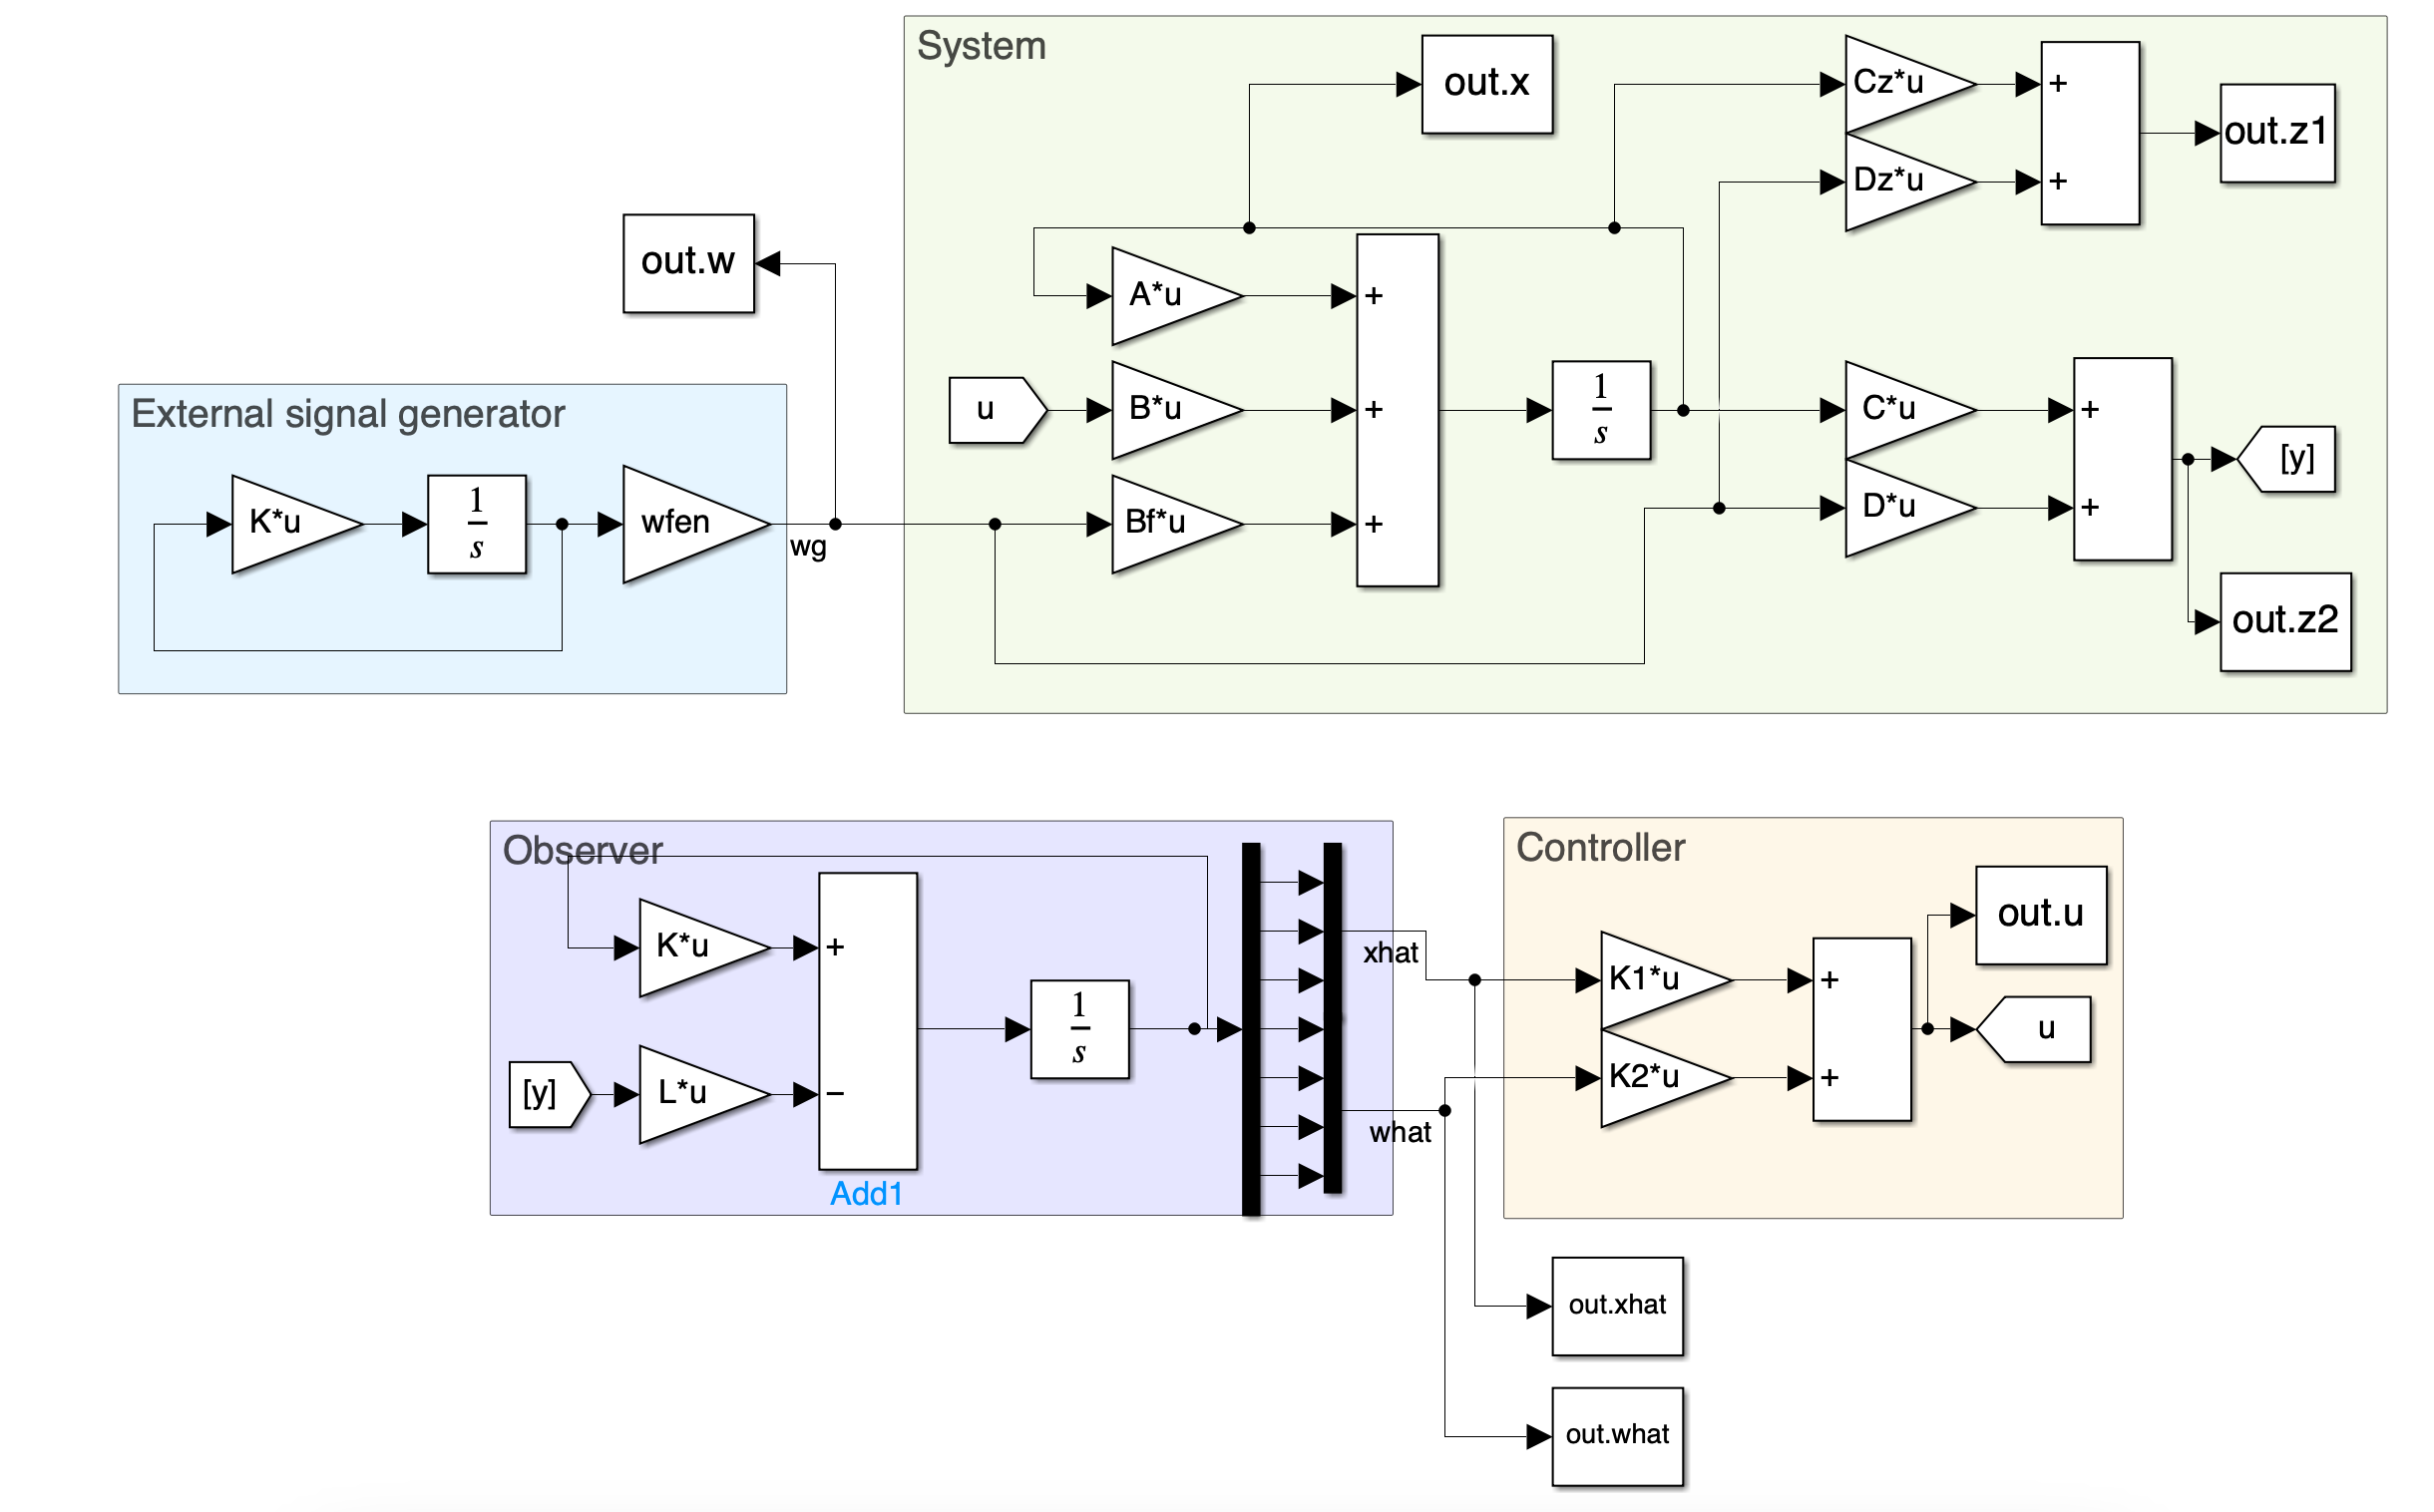
\includegraphics[width=\textwidth]{media/scheme3.png}
    \caption{Схема моделирования системы}
    \label{fig:scheme3}
\end{figure}

\subsection{Анализ внешнего возмущения}
Согласно результатам, полученным ранее, входное воздействие представляет собой 
гармонический сигнал, состоящий из двух частот. График входного воздействия
представлен на рисунке \ref{fig:wf}.

\subsection{Анализ системы}
Рассмотрим \textit{объединенную} систему, которая включает в себя как 
вектор состояния, так и вектор внешнего возмущения. Определим обнаруживаемость пары (блочной матрицы) 
\begin{eqnarray}
    \left(\begin{bmatrix}
        C & D
    \end{bmatrix}, \begin{bmatrix}
        A & B_f \\ 
        0 & \Gamma
    \end{bmatrix}\right) 
\end{eqnarray}
Для этого найдем ее матрицу обнуруживаемости и определим ее ранг. 
\begin{equation}
    W = \begin{bmatrix}
        8.00  & 1.00  & 11.00  & 0.00  & 1.00  & -1.00  & -1.00 \\ 
        4.00  & 0.00  & 4.00  & 0.00  & 0.00  & 0.00  & 0.00 \\ 
        -4.00  & -3.00  & -7.00  & 0.00  & -1.00  & 0.00  & 0.00 \\ 
        0.00  & 0.00  & 0.00  & -40.00  & 16.00  & 9.00  & 7.00 \\ 
        0.00  & 0.00  & 0.00  & -64.00  & 25.00  & 14.00  & 12.00 \\ 
        0.00  & 0.00  & 0.00  & -26.00  & 11.00  & 7.00  & 3.00 \\ 
        0.00  & 0.00  & 0.00  & -48.00  & 18.00  & 14.00  & 8.00 \\ 
    \end{bmatrix}
\end{equation}
\begin{equation}
    \text{rank}(W) = 7 = \text{dim}(W)
\end{equation}
Таким образом, система является наблюдаемой, так как ранг матрицы обнаруживаемости равен
размерности матрицы. Значит можно реализовать слежение и компенсацию по выходу.

\subsection{Расширенный наблюдатель}
Рассмотрим уравнение расширенного наблюдателя 
\begin{equation}
    \begin{bmatrix}
        \dot{\hat{x}} \\ 
        \dot{\hat{w}} \\
    \end{bmatrix} = \overline{A} 
    \begin{bmatrix}
        \hat{x} \\ 
        \hat{w} \\
    \end{bmatrix} - Ly
    \label{eq:extended_observer}
\end{equation}
Подставив в него матрицы системы, получим
\begin{eqnarray}
    \overline{A} = \begin{bmatrix}
       A + BK_1 + L_1 C & BK_2 + B_f + L_1 D \\ 
       L_2 C & \Gamma + L_2 D \\
    \end{bmatrix}
\end{eqnarray}
Далее найдем недостающие компоненты. Оценку данным наблюдателем будем 
использовать для создания регулятора вида 
\begin{equation}
    u = K_1 \hat{x} + K_2 \hat{w} 
\end{equation}

\subsection{Синтез регулятора}
\subsubsection{Feedback компонента}
В силу неизменности матриц, задающих систему, регулятор $K_1$, 
полученный ранее остается прежним. 
\begin{equation}
    K_1 = \begin{bmatrix}
        -4.57  & 0.29  & -4.57 \\ 
    \end{bmatrix}
\end{equation}
\subsubsection{Синтез наблюдателя}
Синтезируем наблюдатель с заданной степенью устойчивости $\alpha = 3$ и минимизаций нормы управления
используя матричные неравенства Ляпунова, аналогично синтезу регулятора, рассмотренного ранее. 
Получим матрицу $L$:
\begin{equation}
    L = \begin{bmatrix}
        -14.41 \\ 
        -2.37 \\ 
        12.45 \\ 
        -50.07 \\ 
        -77.47 \\ 
        -49.82 \\ 
        -65.29 \\ 
    \end{bmatrix}
\end{equation}
Согласно уравнению \ref{eq:extended_observer}, первые три элемента матрицы $L$
соответствуют матрице $L_1$, а последние четыре элемента матрицы $L_2$ -- 
матрице оценки системы и внешнего возмущения соответственно.
Таким образом,
\begin{equation}
    \begin{array}{cc}
        L_1 = \begin{bmatrix}
            -14.41 & -2.37 & 12.45
        \end{bmatrix}^T, &
        L_2 = \begin{bmatrix}
            -50.07 & -77.47 & -49.82 & -65.29
        \end{bmatrix}^T
    \end{array}
\end{equation}
\subsubsection{Feedforward компонента}
Для синтеза следящего регулятора c виртуальным выходом $z_1 = C_zx + D_z w$ воспользуемся уравнениями: 
\begin{equation}
    \begin{cases}
        P\Gamma - AP = BY + B_f \\
        C_z P + D_z = 0 \\ 
        K_2 = Y - K_1 P \\ 
    \end{cases}
\end{equation}
Решая систему уравнений, получаем регулятор $K_{21}$: 
\begin{equation}
    K_{21} = \begin{bmatrix}
        -2.57  & 1.28  & 5.08  & -1.30 \\ 
    \end{bmatrix}    
\end{equation}
Для синтеза следящего регулятора c виртуальным выходом $z_2 = y$ воспользуемся уравнениями:
\begin{equation}
    \begin{cases}
        P\Gamma - AP = BY + B_f \\
        C P + D = 0 \\ 
        K_2 = Y - K_1 P \\ 
    \end{cases}
\end{equation}
Решая систему уравнений, получаем регулятор $K_{22}$:
\begin{equation}
    K_{22} = \begin{bmatrix}
        -6.54  & 1.53  & 4.35  & 1.82 \\ 
    \end{bmatrix}
\end{equation}

\subsection{Моделирование}
Теперь, когда все компоненты расширенного наблюдателя (\ref{eq:extended_observer}) известны, 
можно смоделировать системы с полученными регуляторами и наблюдателем. При этом полученная матрица 
наблюдателя $\overline{A}$ будет иметь вид для виртуального выхода $z_1$:
\begin{equation}
    \overline{A} = \begin{bmatrix}
        41.39  & 43.94  & 29.98  & 175.40  & -28.99  & -35.23  & -86.06 \\ 
        22.44  & 6.24  & 20.08  & 35.91  & -8.25  & -20.96  & -10.02 \\ 
        -42.60  & -39.48  & -33.16  & -156.87  & 27.41  & 41.12  & 70.50 \\ 
        100.15  & 150.22  & 50.07  & 560.87  & -84.15  & -91.15  & -293.44 \\ 
        154.95  & 232.42  & 77.47  & 865.68  & -129.95  & -140.95  & -452.84 \\ 
        99.63  & 149.45  & 49.82  & 571.78  & -88.63  & -92.63  & -295.89 \\ 
        130.59  & 195.88  & 65.29  & 735.53  & -112.59  & -116.59  & -383.77 \\ 
    \end{bmatrix}
\end{equation}
и ее собственные числа: 
\begin{equation}
    \sigma(\overline{A}) = \begin{bmatrix}
        -14.68 + 37.26j \\ 
        -14.68 - 37.26j \\ 
        0.09 + 3.69j \\ 
        0.09 - 3.69j \\ 
        0.59 + 2.00j \\ 
        0.59 - 2.00j \\ 
        -3.00 \\ 
    \end{bmatrix}
\end{equation}
и для виртуального выхода $z_2$:
\begin{equation}
    \overline{A} = \begin{bmatrix}
        41.39  & 43.94  & 29.98  & 179.86  & -29.44  & -34.29  & -89.43 \\ 
        22.44  & 6.24  & 20.08  & 49.29  & -9.61  & -18.16  & -20.13 \\ 
        -42.60  & -39.48  & -33.16  & -170.25  & 28.77  & 38.32  & 80.62 \\ 
        100.15  & 150.22  & 50.07  & 560.87  & -84.15  & -91.15  & -293.44 \\ 
        154.95  & 232.42  & 77.47  & 865.68  & -129.95  & -140.95  & -452.84 \\ 
        99.63  & 149.45  & 49.82  & 571.78  & -88.63  & -92.63  & -295.89 \\ 
        130.59  & 195.88  & 65.29  & 735.53  & -112.59  & -116.59  & -383.77 \\ 
    \end{bmatrix}
\end{equation}
\begin{equation}
    \sigma(\overline{A}) = \begin{bmatrix}
        -14.00 + 35.43j \\ 
        -14.00 - 35.43j \\ 
        0.00 + 3.00j \\ 
        0.00 - 3.00j \\ 
        -0.00 + 2.00j \\ 
        -0.00 - 2.00j \\ 
        -3.00 \\ 
    \end{bmatrix}
\end{equation}
В первом спектре присутствуют неустойчивый собственные числа, что указывает на то, что в 
спектре есть компоненты от неустойчивого входного воздействия, но при этом эти компоненты не 
совпадают с собственными числами генератора возмущения. Во втором спектре же есть точное 
совпадение с собственными числами генератора возмущения, что указывает на то, что система
содержит в себе полную модель. Выход, построенный на таком генераторе может полностью и точно 
компенсировать входное воздействие. 

Сравнительный график реального состояния системы и его оценки для виртуального выхода $z_1$
представлен на рисунке \ref{fig:task3_z2_x_cmp}, сравнение внешнего возмущения
и его оценки представлено на рисунке \ref{fig:task3_z2_w_cmp}.
\begin{figure}[ht!]
    \centering
    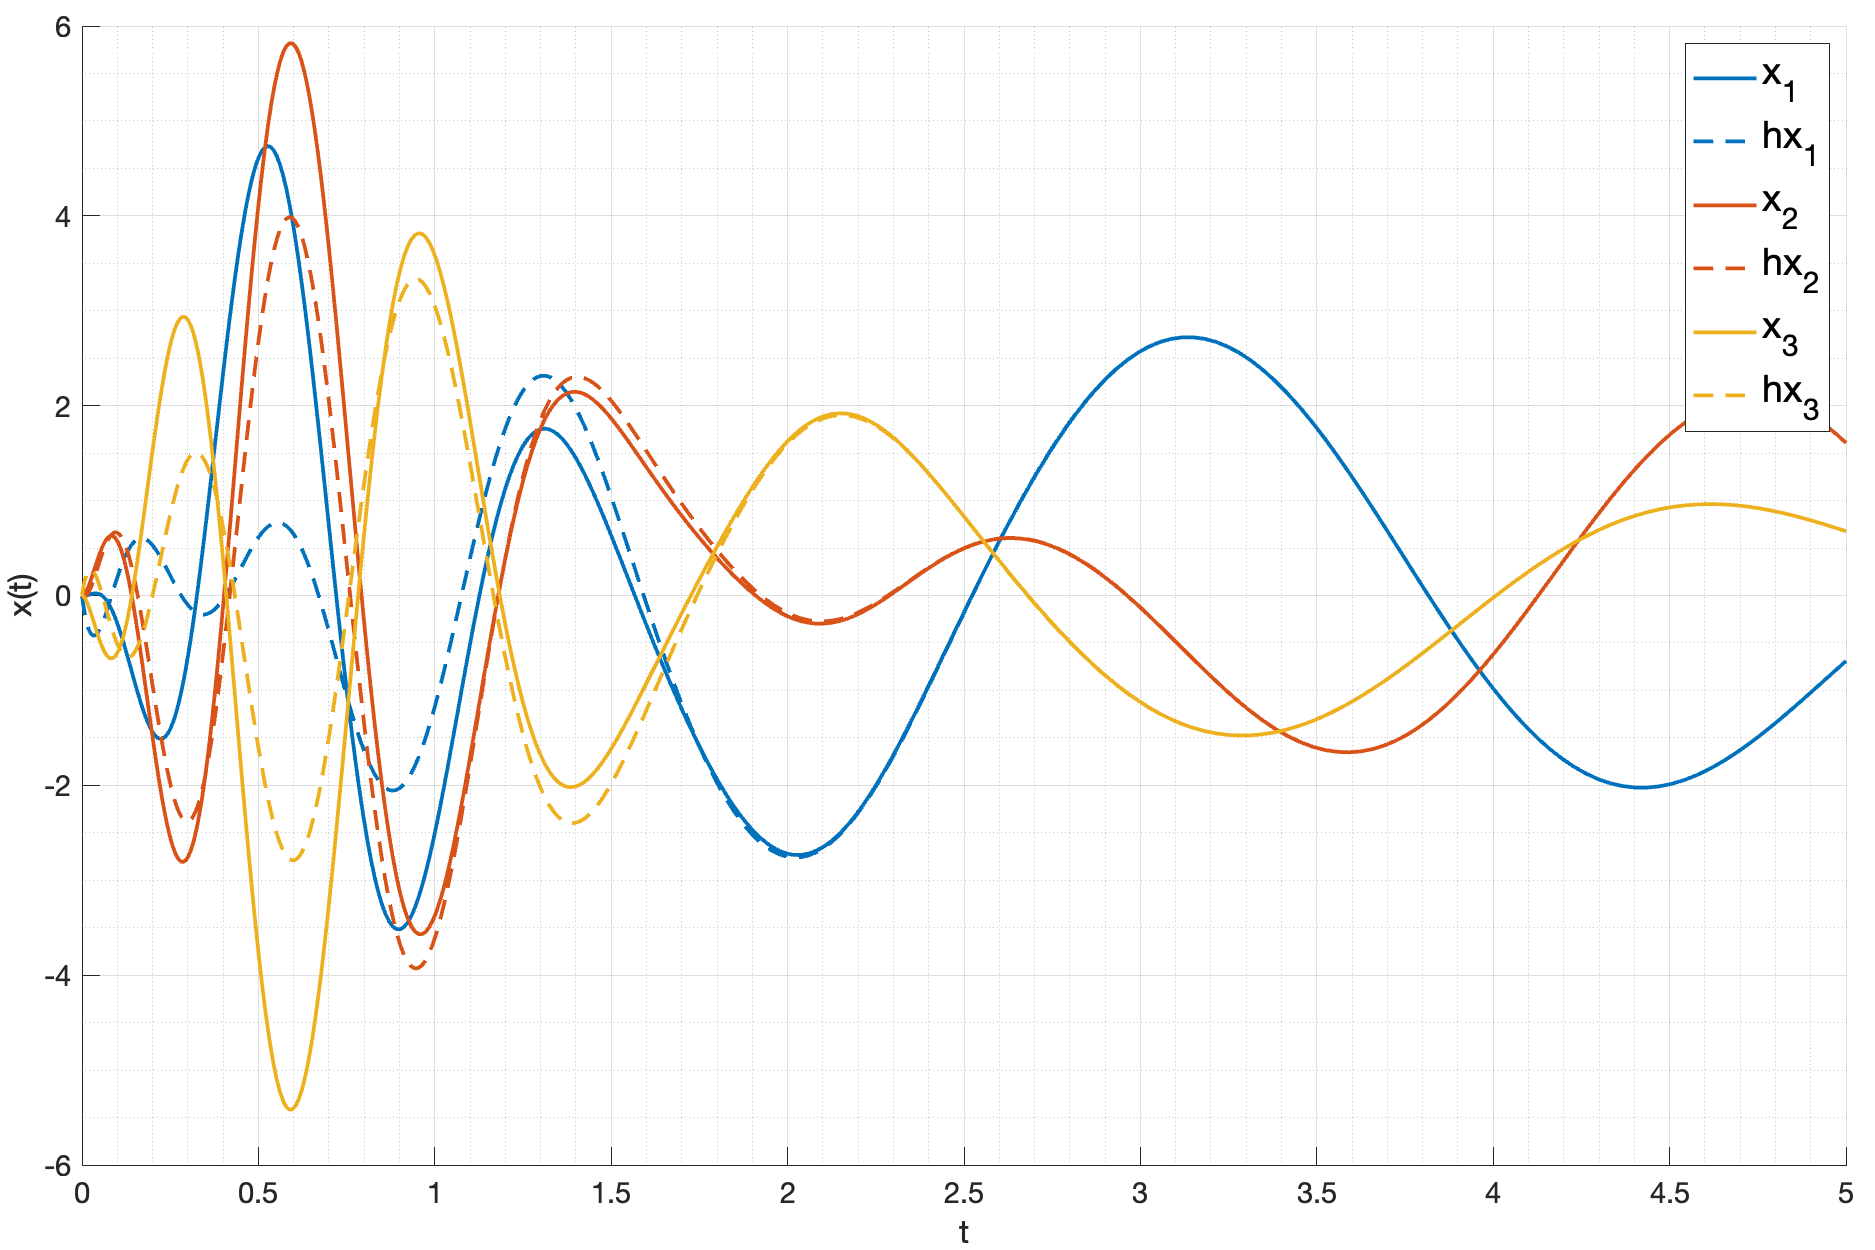
\includegraphics[width=\textwidth]{media/plots/task3_z2_x_cmp.png}
    \caption{Сравнение состояния системы и его оценки}
    \label{fig:task3_z2_x_cmp}
\end{figure}
\begin{figure}[ht!]
    \centering
    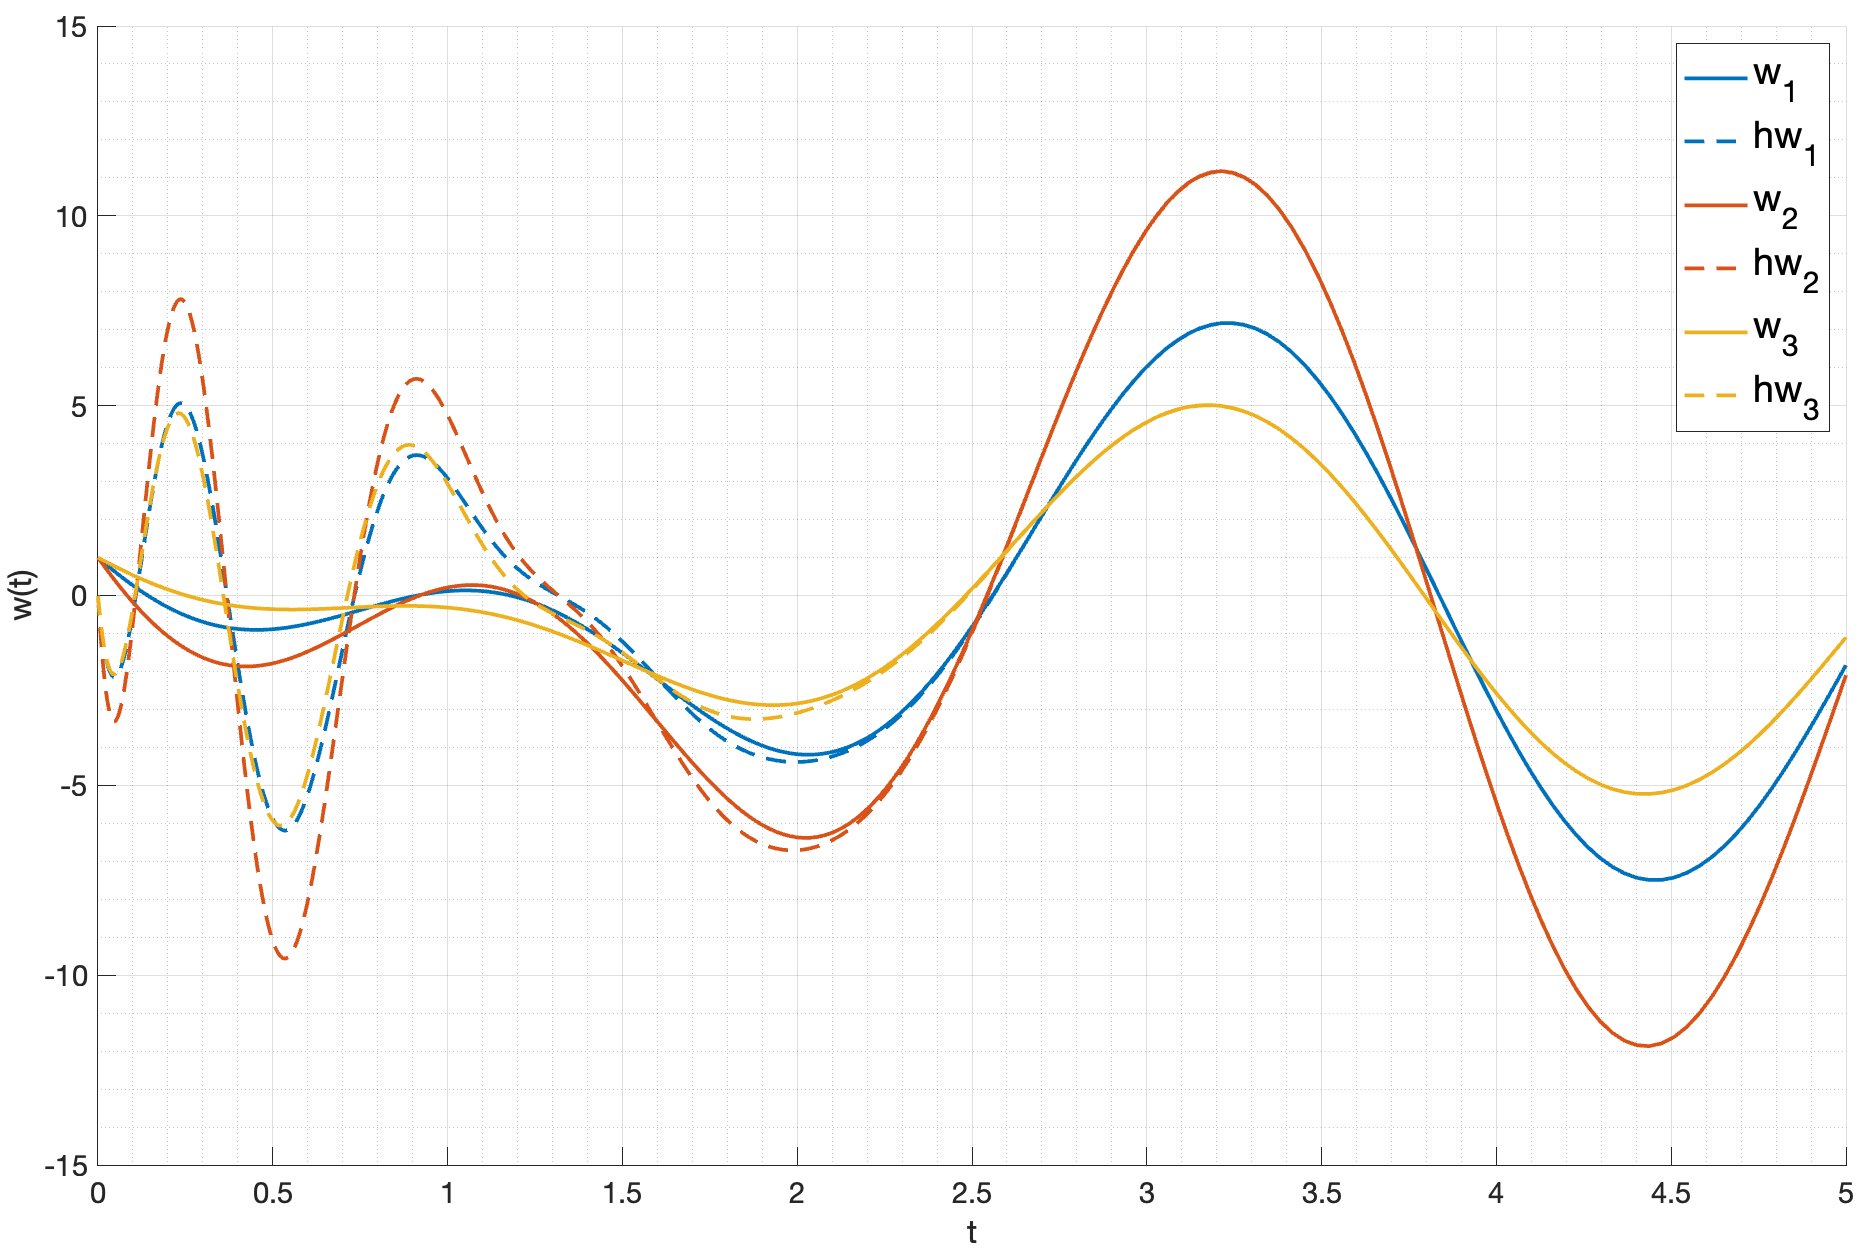
\includegraphics[width=\textwidth]{media/plots/task3_z2_w_cmp.png}
    \caption{Сравнение внешнего возмущения и его оценки}
    \label{fig:task3_z2_w_cmp}
\end{figure}
Видно, что обе оценки сходятся к реальным значениям. Убедимся в этом, посмотрев на график
ошибки наблюдения на рисунке \ref{fig:task3_z2_xerr_cmp} и \ref{fig:task3_z2_werr_cmp} (для оценки состояния и внешнего возмущения соответственно).
\begin{figure}[ht!]
    \centering
    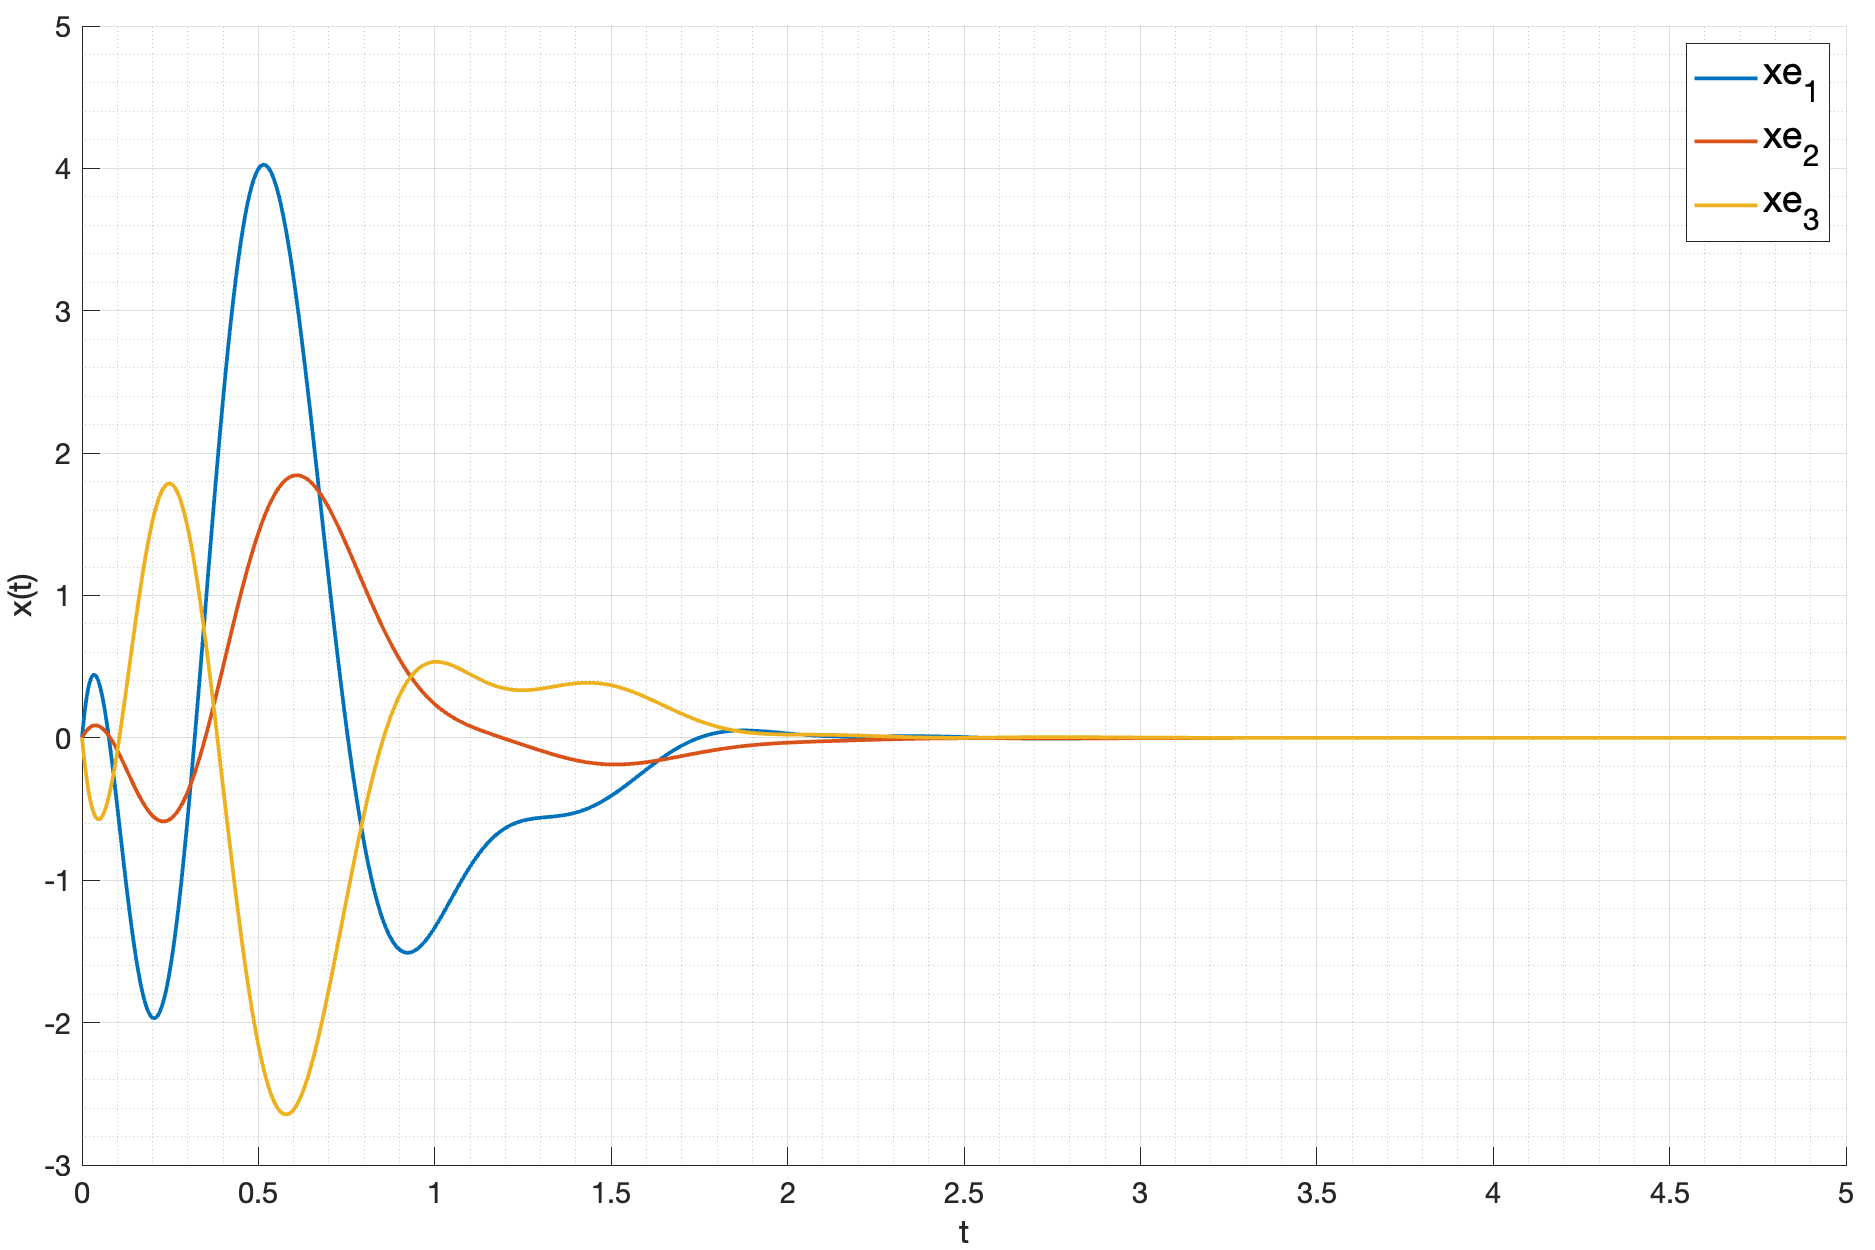
\includegraphics[width=\textwidth]{media/plots/task3_z2_xerr_cmp.png}
    \caption{Ошибка наблюдения состояния системы}
    \label{fig:task3_z2_xerr_cmp}
\end{figure}
\begin{figure}[ht!]
    \centering
    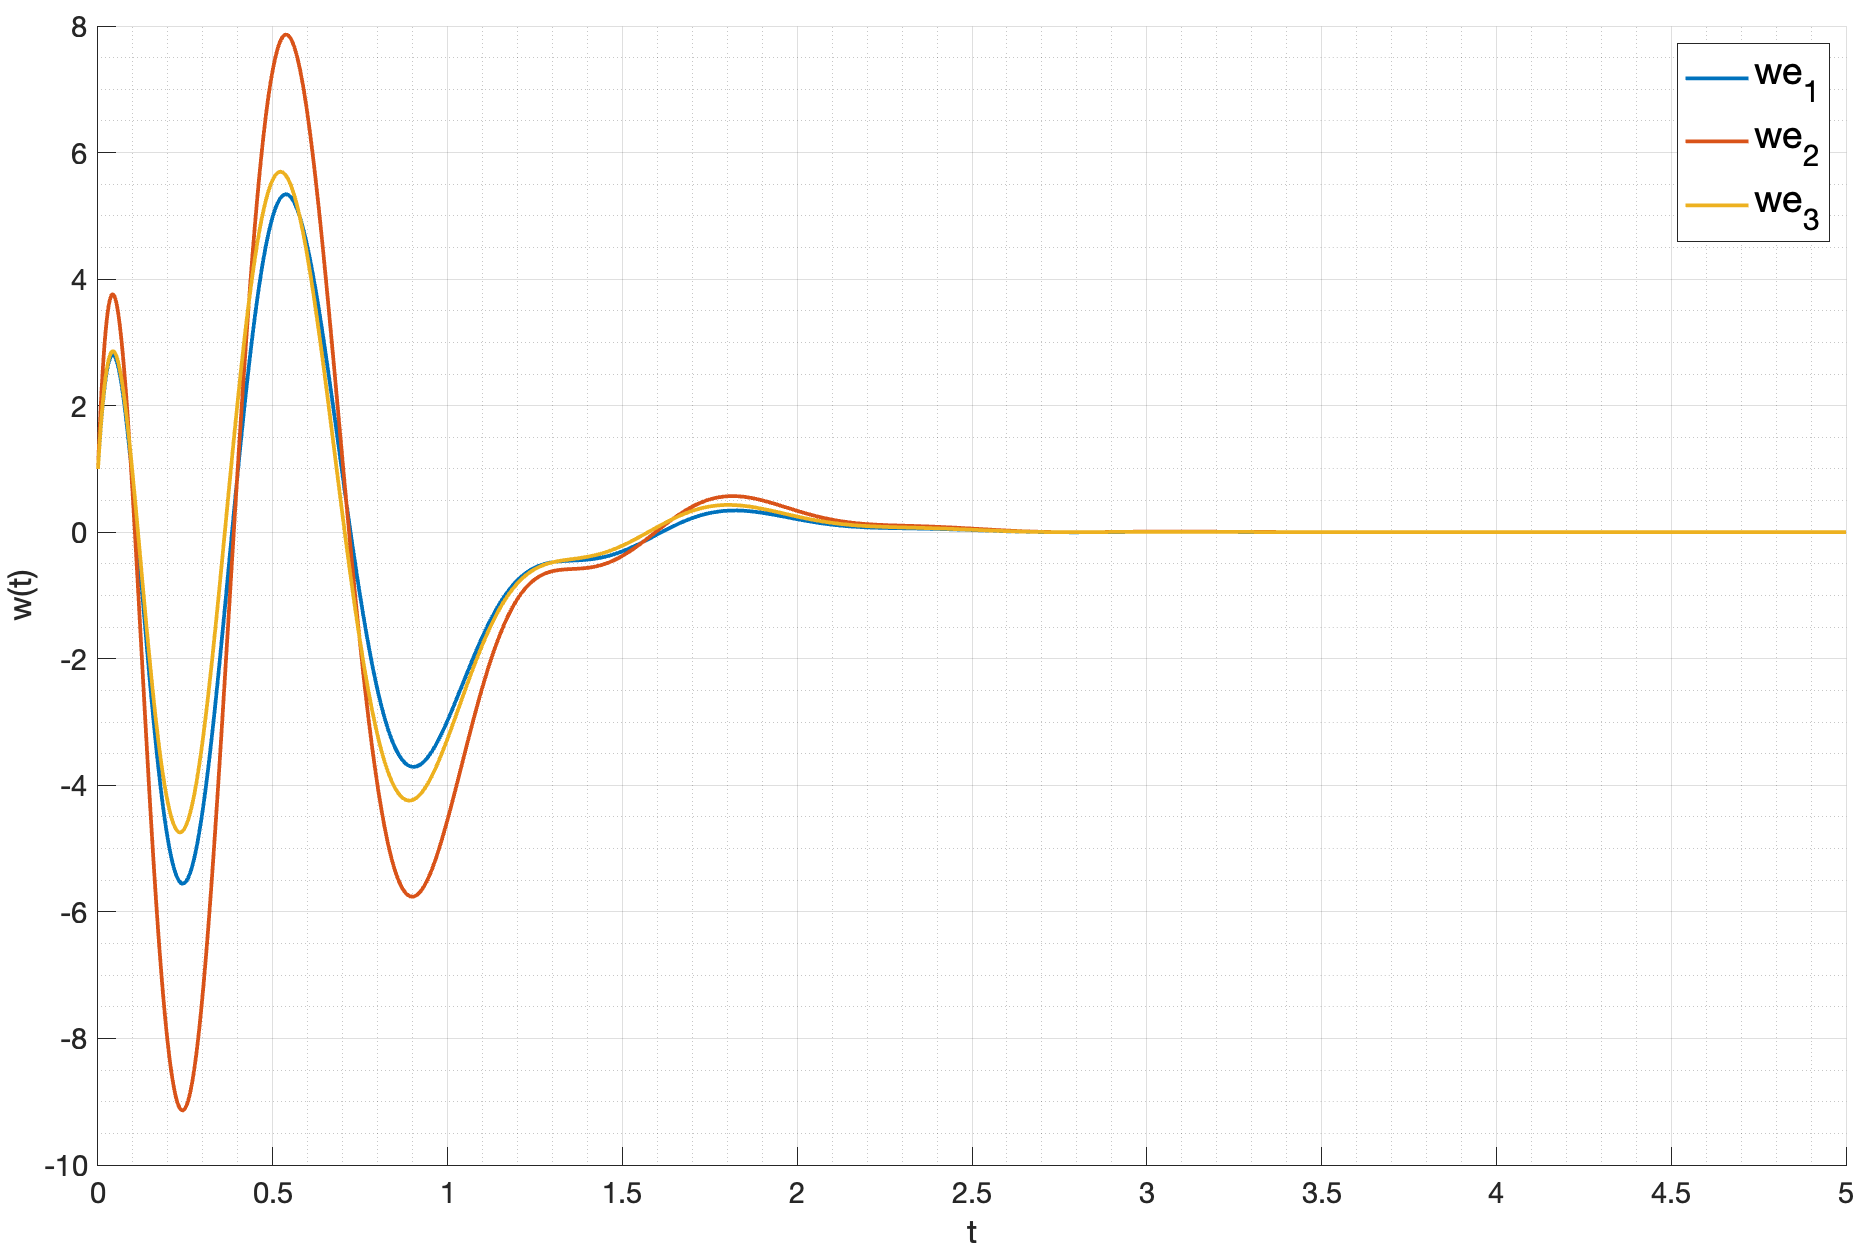
\includegraphics[width=\textwidth]{media/plots/task3_z2_werr_cmp.png}
    \caption{Ошибка наблюдения внешнего возмущения}
    \label{fig:task3_z2_werr_cmp}
\end{figure}
Обе ошибки наблюдения стремятся к нулю, что подтверждает корректность синтеза. 

Сравнительный график фактического и виртуального выхода системы представлен на рисунке \ref{fig:task3_z1_cmp} ($z_1$ -- виртуальный выход, $z_2$ -- фактический выход).
\begin{figure}[ht!]
    \centering
    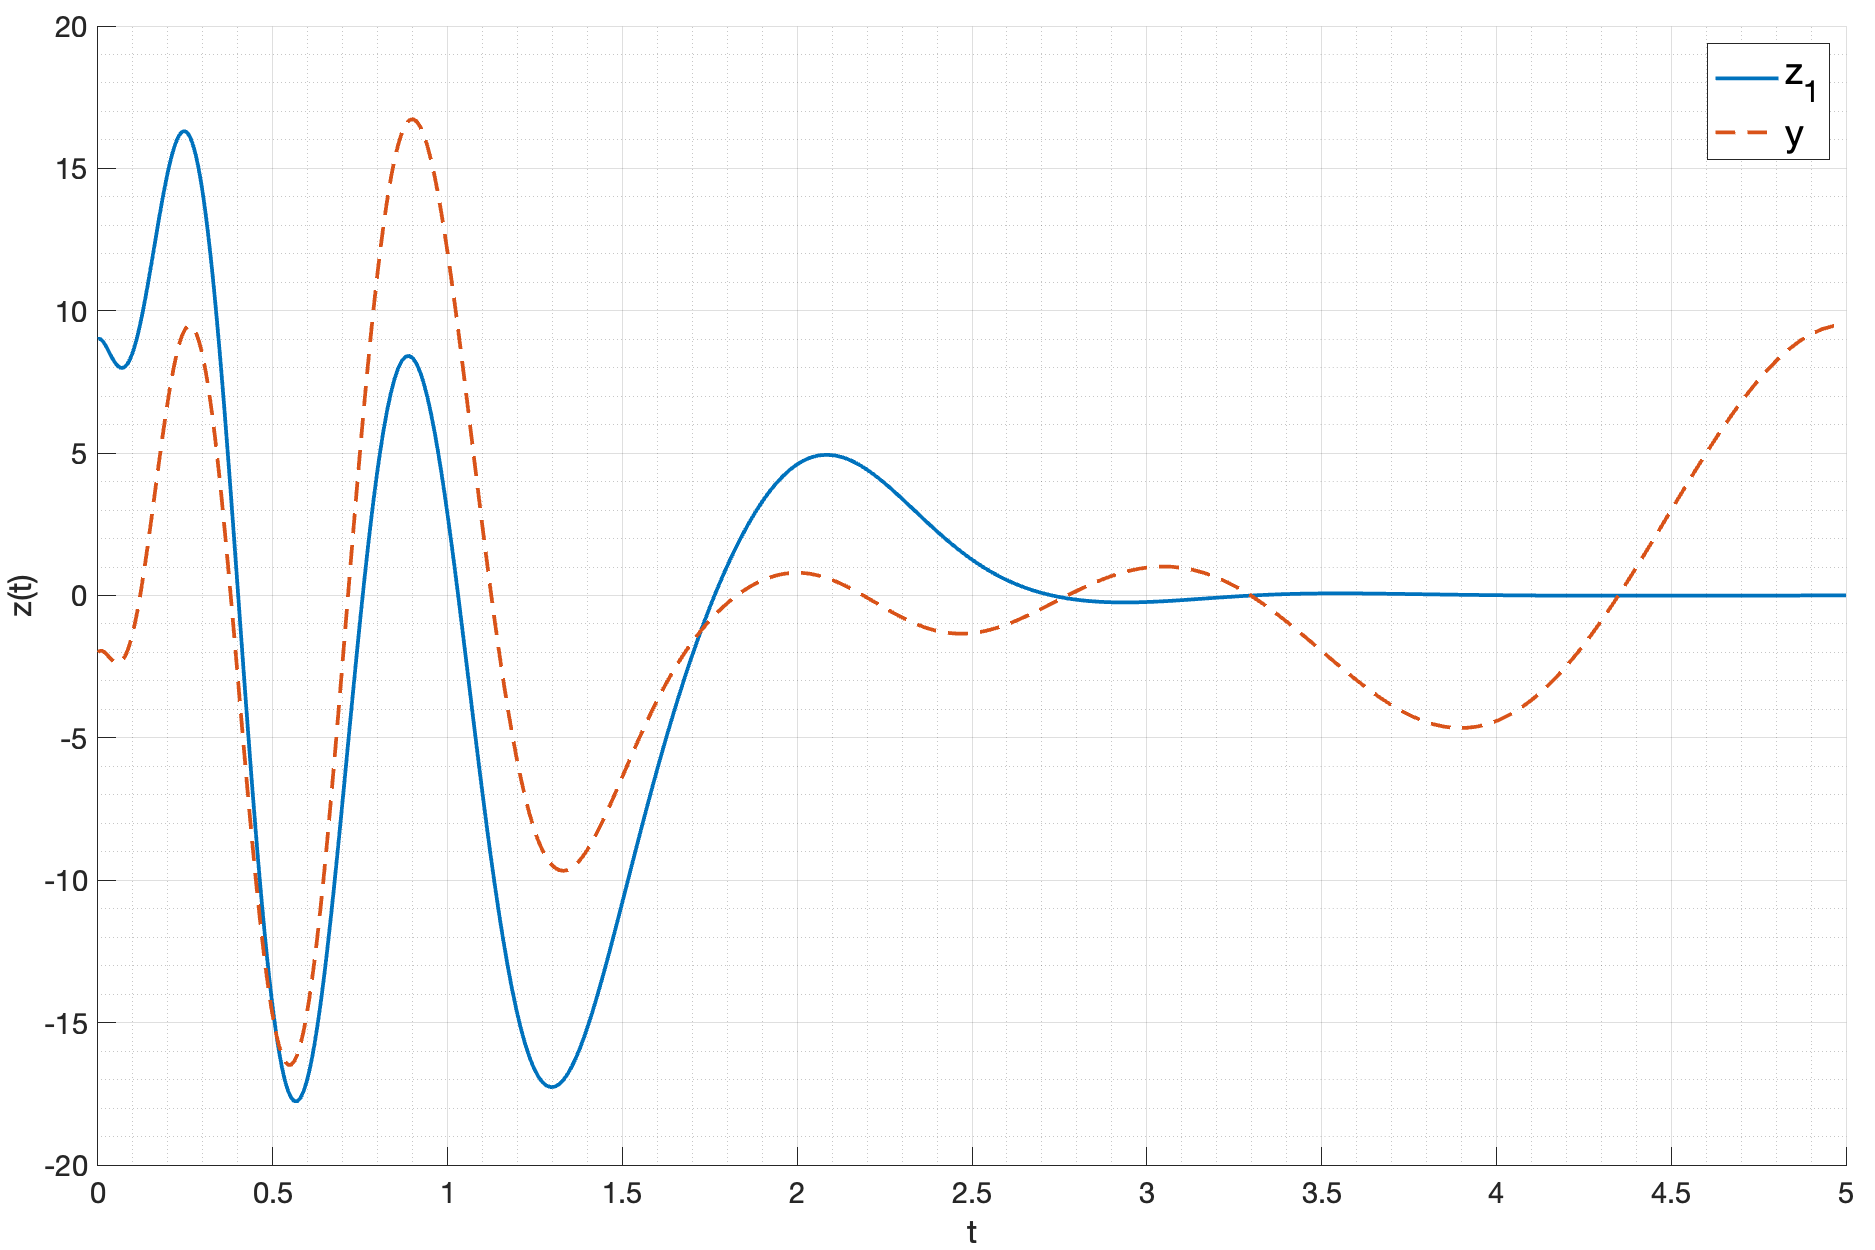
\includegraphics[width=\textwidth]{media/plots/task3_z1_cmp.png}
    \caption{Сравнение фактического и виртуального выхода системы}
    \label{fig:task3_z1_cmp}
\end{figure}
Видно, что фактический и виртуальный выходы система не совпадают, что связано с тем, как отмечалось 
ранее, что собственные числа генератора не входят в спектр наблюдателя. 

\FloatBarrier
Сравнительный график состояния системы и его оценки для виртуального выхода $z_2$
представлен на рисунке \ref{fig:task3_z2_x_cmp}, сравнение внешнего возмущения
и его оценки представлено на рисунке \ref{fig:task3_z2_w_cmp}.
\begin{figure}[ht!]
    \centering
    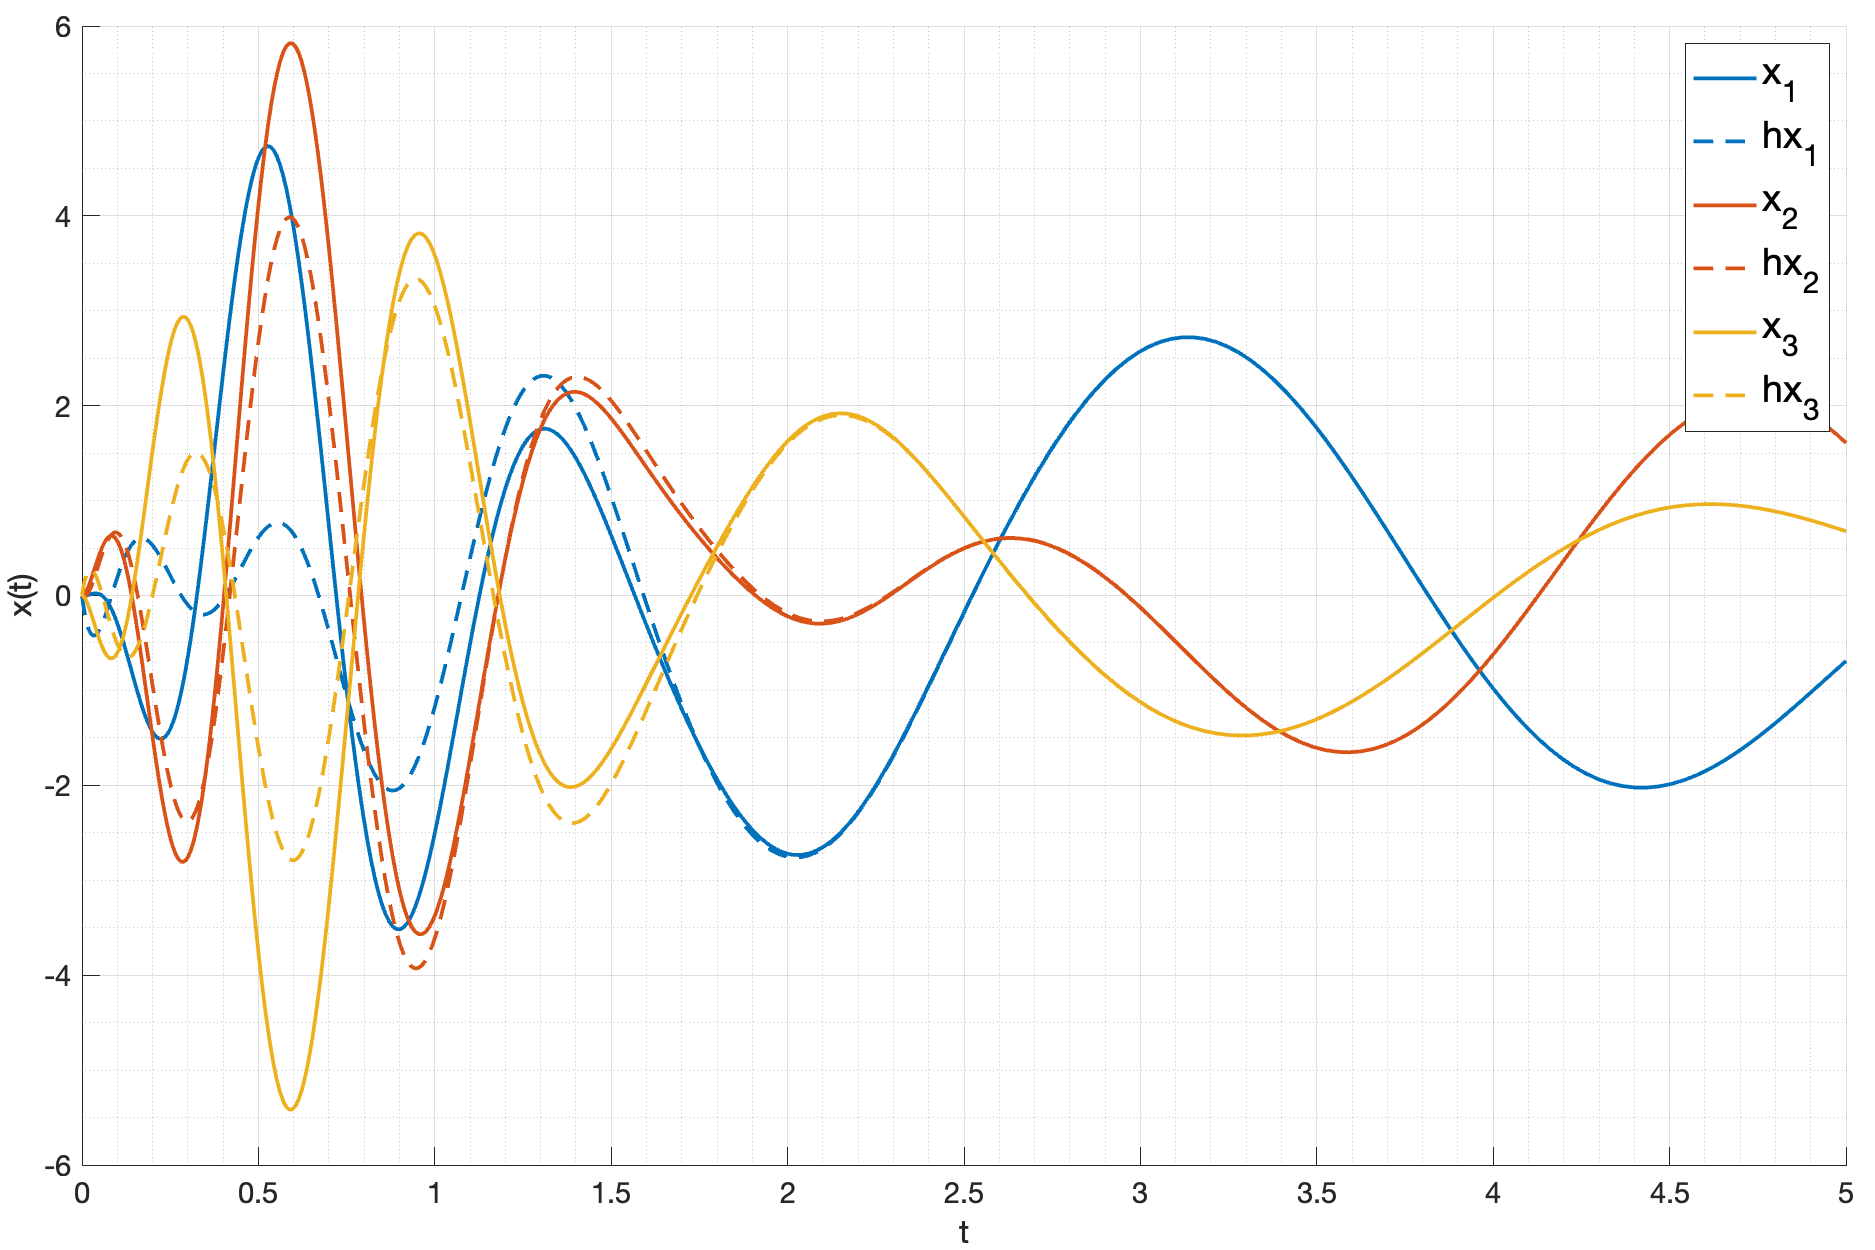
\includegraphics[width=\textwidth]{media/plots/task3_z2_x_cmp.png}
    \caption{Сравнение состояния системы и его оценки}
    \label{fig:task3_z2_x_cmp}
\end{figure}
\begin{figure}[ht!]
    \centering
    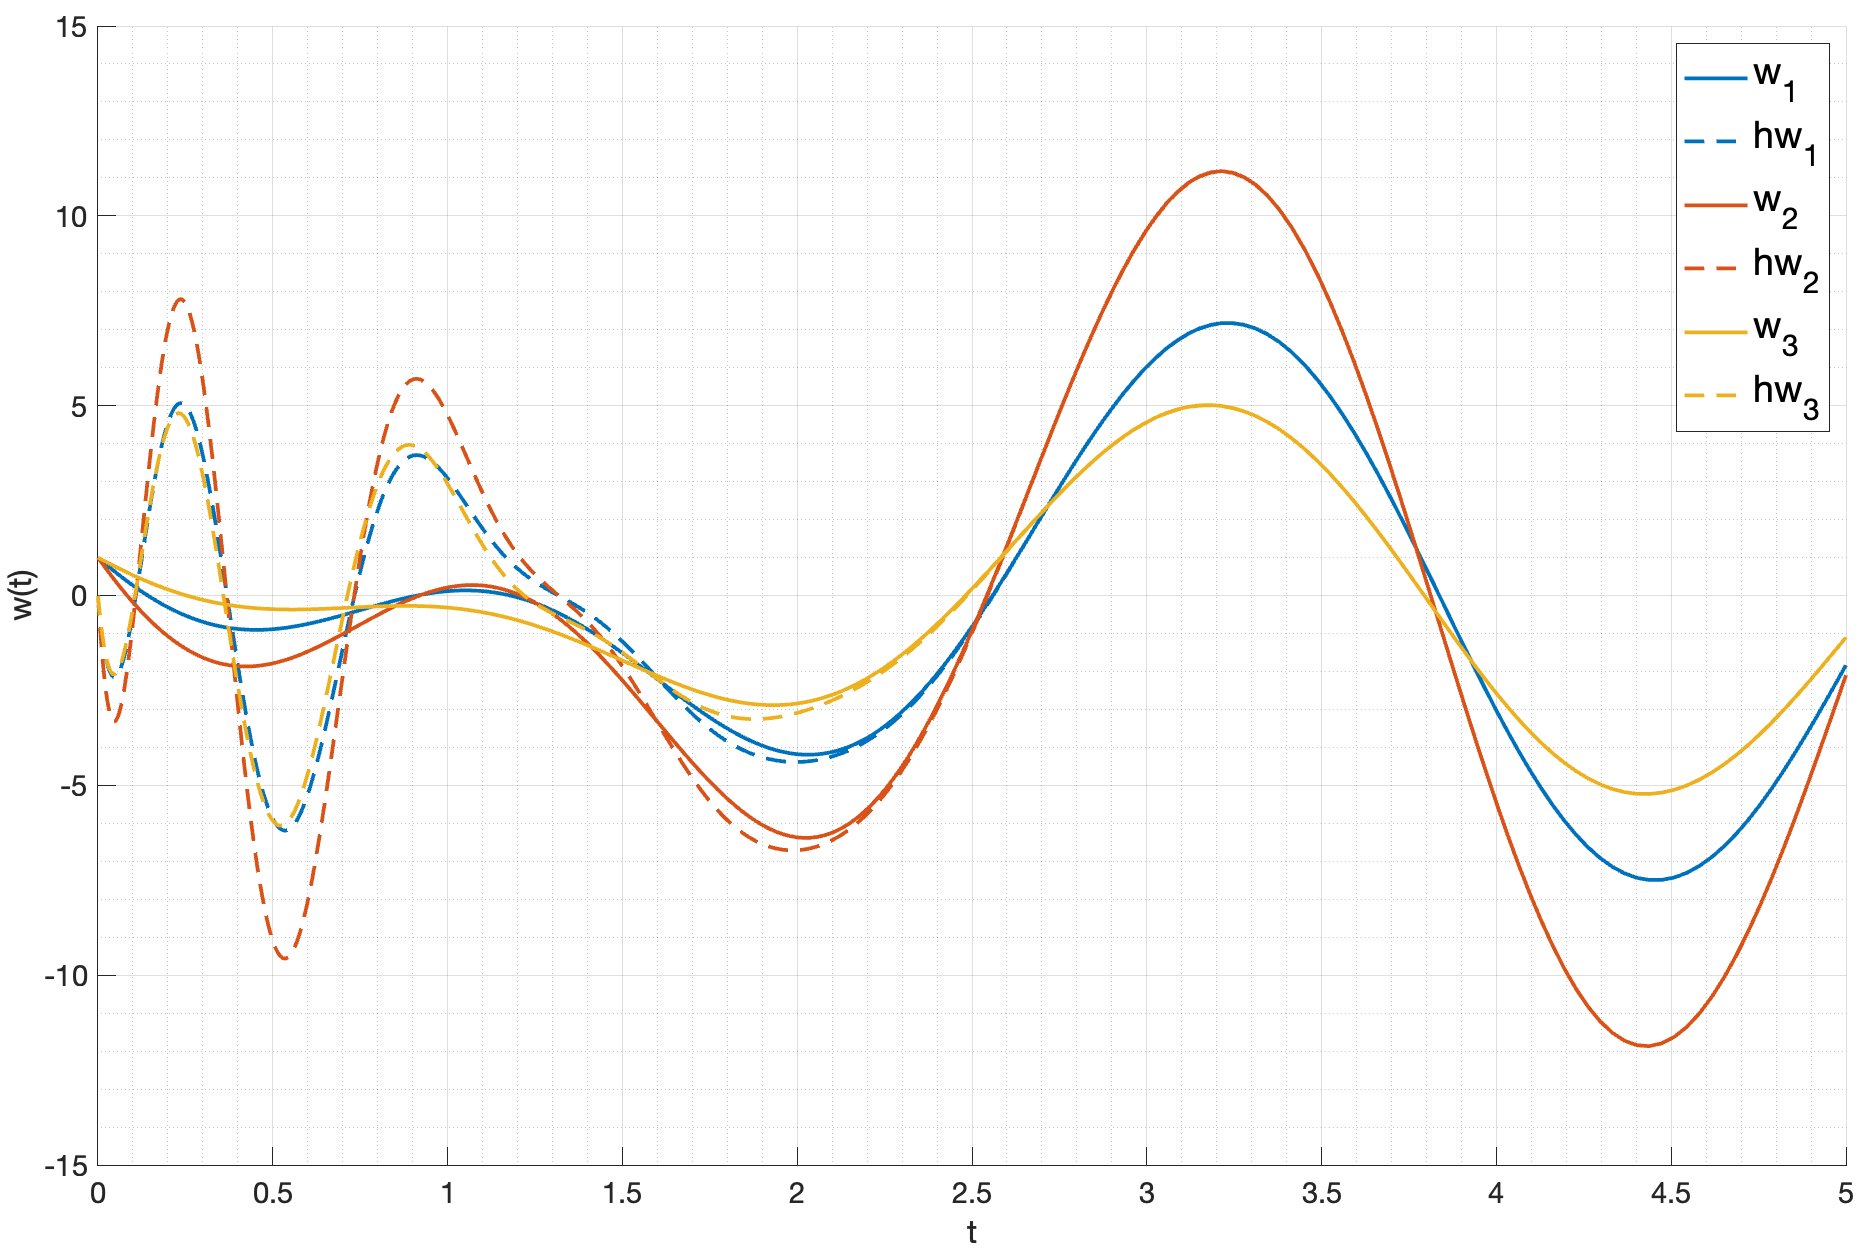
\includegraphics[width=\textwidth]{media/plots/task3_z2_w_cmp.png}
    \caption{Сравнение внешнего возмущения и его оценки}
    \label{fig:task3_z2_w_cmp}
\end{figure}
Так же, как и в случае с виртуальным выходом $z_1$, видно, что обе оценки сходятся к реальным значениям.
Убедимся в этом, посмотрев на график
ошибки наблюдения на рисунке \ref{fig:task3_z2_xerr_cmp} и \ref{fig:task3_z2_werr_cmp} (для оценки состояния и внешнего возмущения соответственно).
\begin{figure}[ht!]
    \centering
    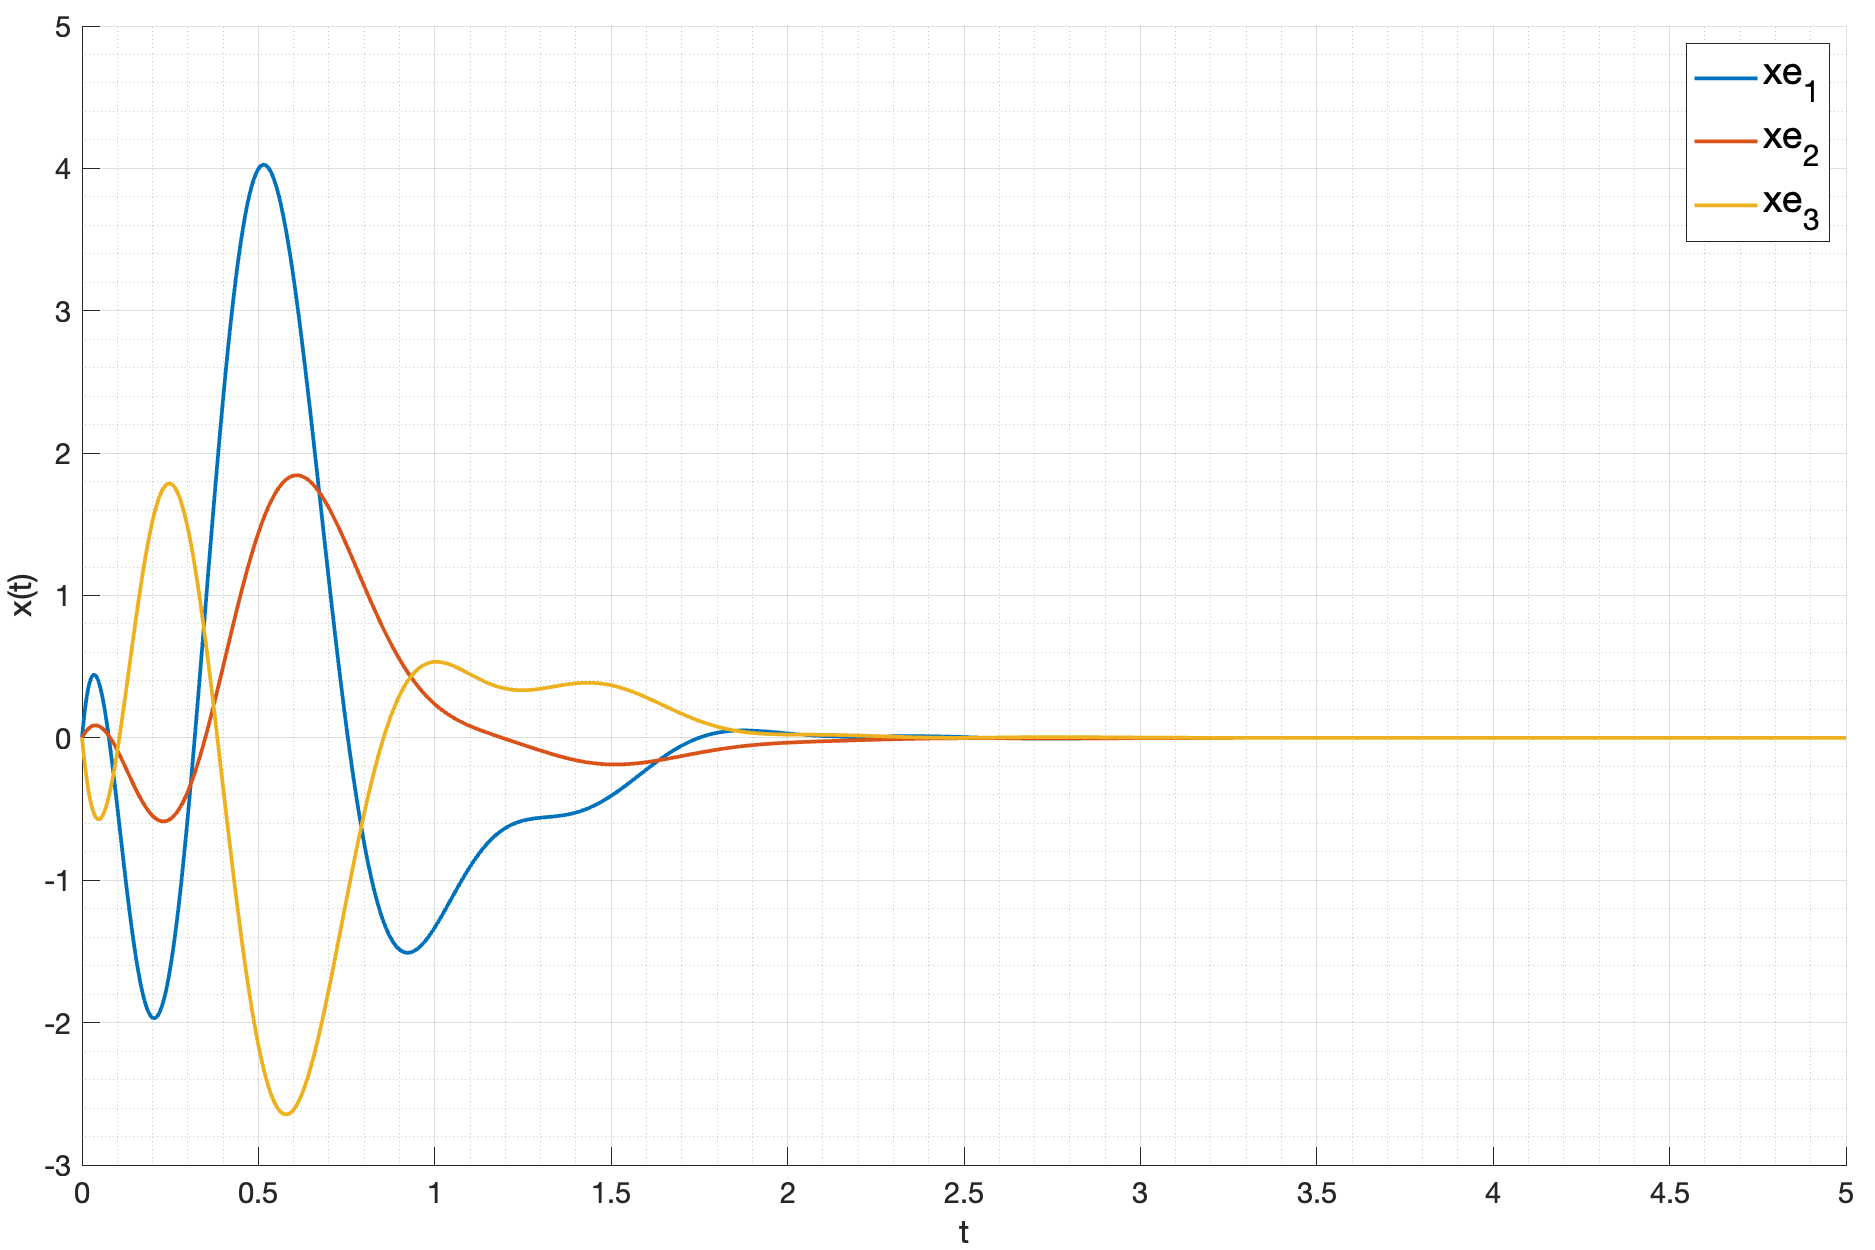
\includegraphics[width=\textwidth]{media/plots/task3_z2_xerr_cmp.png}
    \caption{Ошибка наблюдения состояния системы}
    \label{fig:task3_z2_xerr_cmp}
\end{figure}
\begin{figure}[ht!]
    \centering
    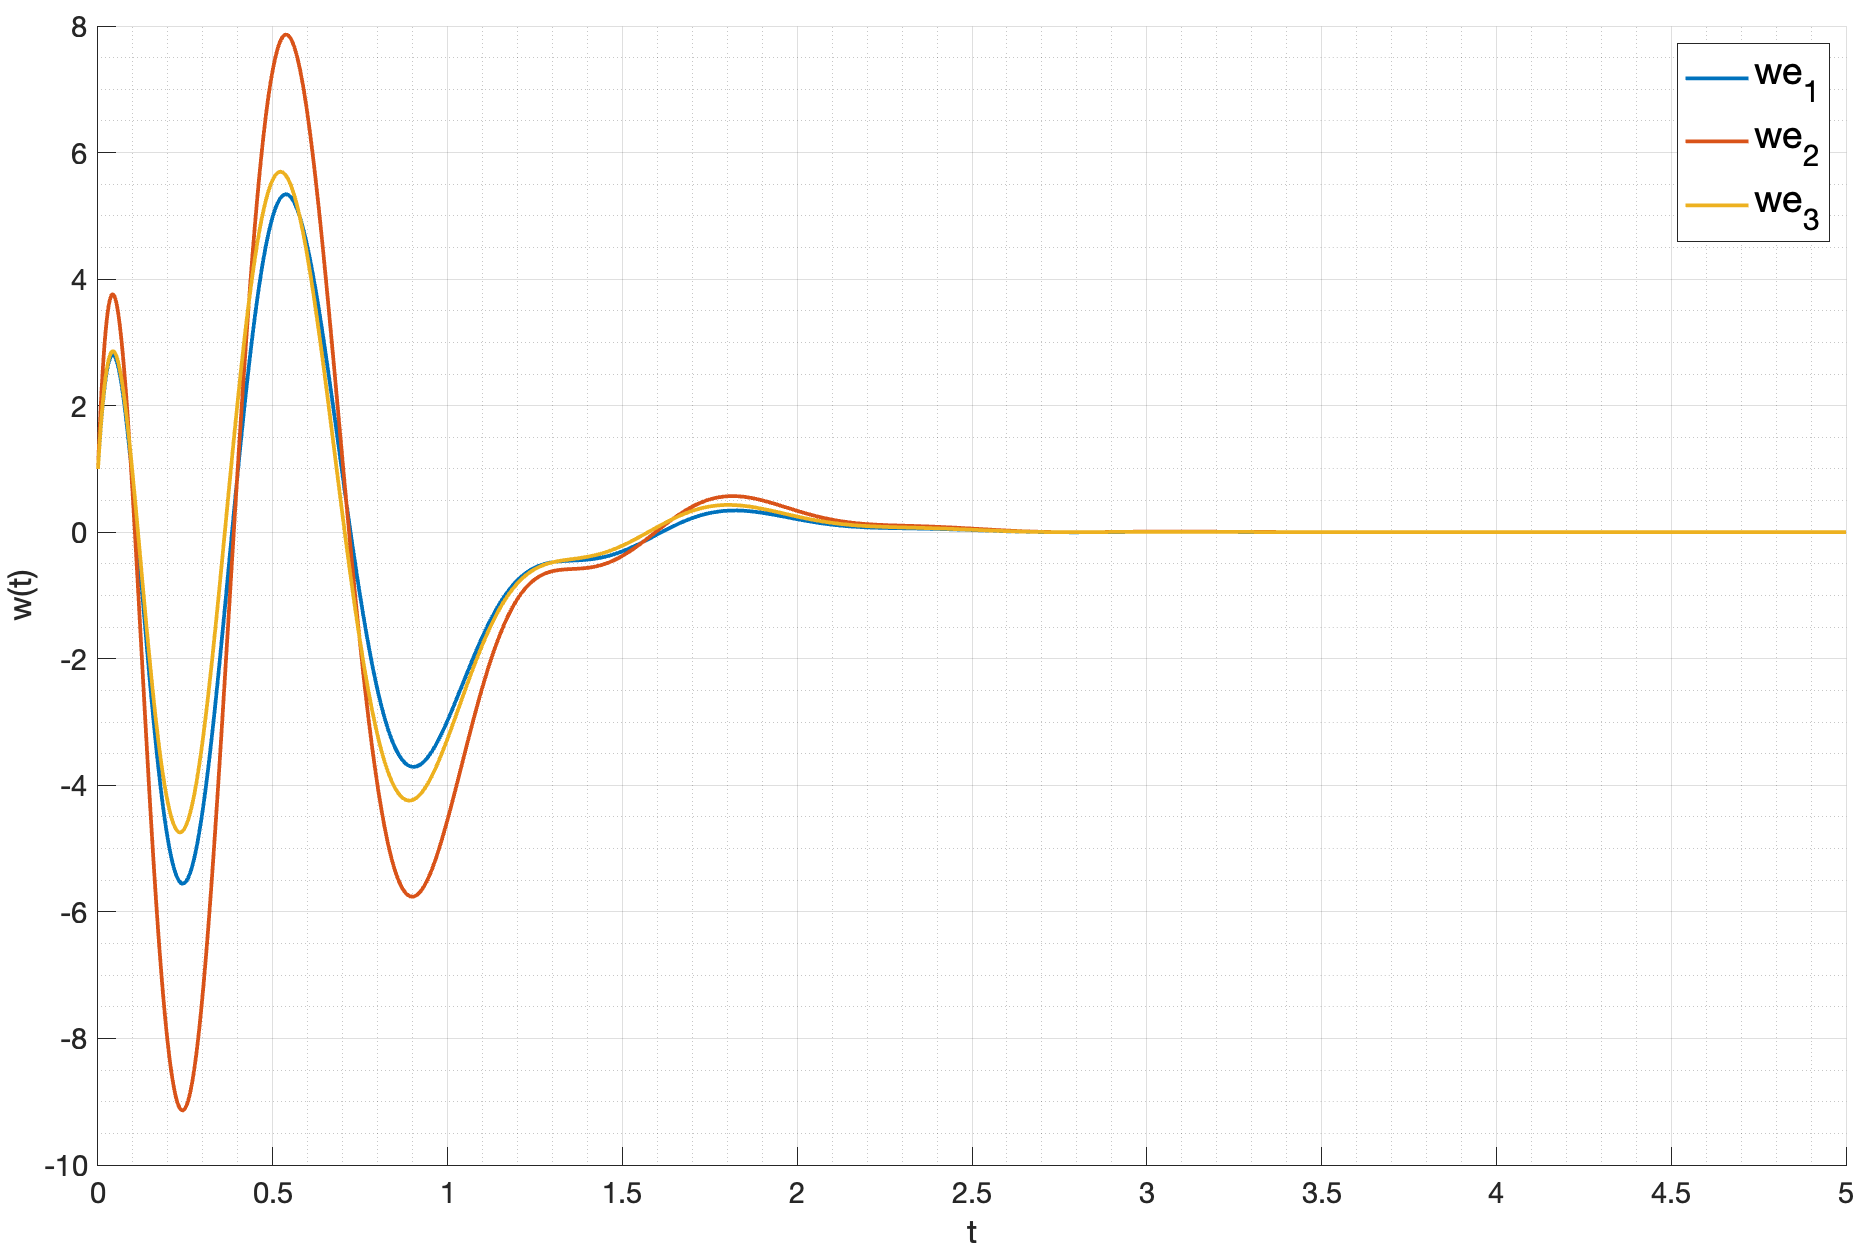
\includegraphics[width=\textwidth]{media/plots/task3_z2_werr_cmp.png}
    \caption{Ошибка наблюдения внешнего возмущения}
    \label{fig:task3_z2_werr_cmp}
\end{figure}
Обе ошибки наблюдения стремятся к нулю, что подтверждает корректность синтеза.
Сравнительный график фактического и виртуального выхода системы представлен на рисунке \ref{fig:task3_z2_cmp} ($z_1$ -- виртуальный выход, $z_2$ -- фактический выход).
\begin{figure}[ht!]
    \centering
    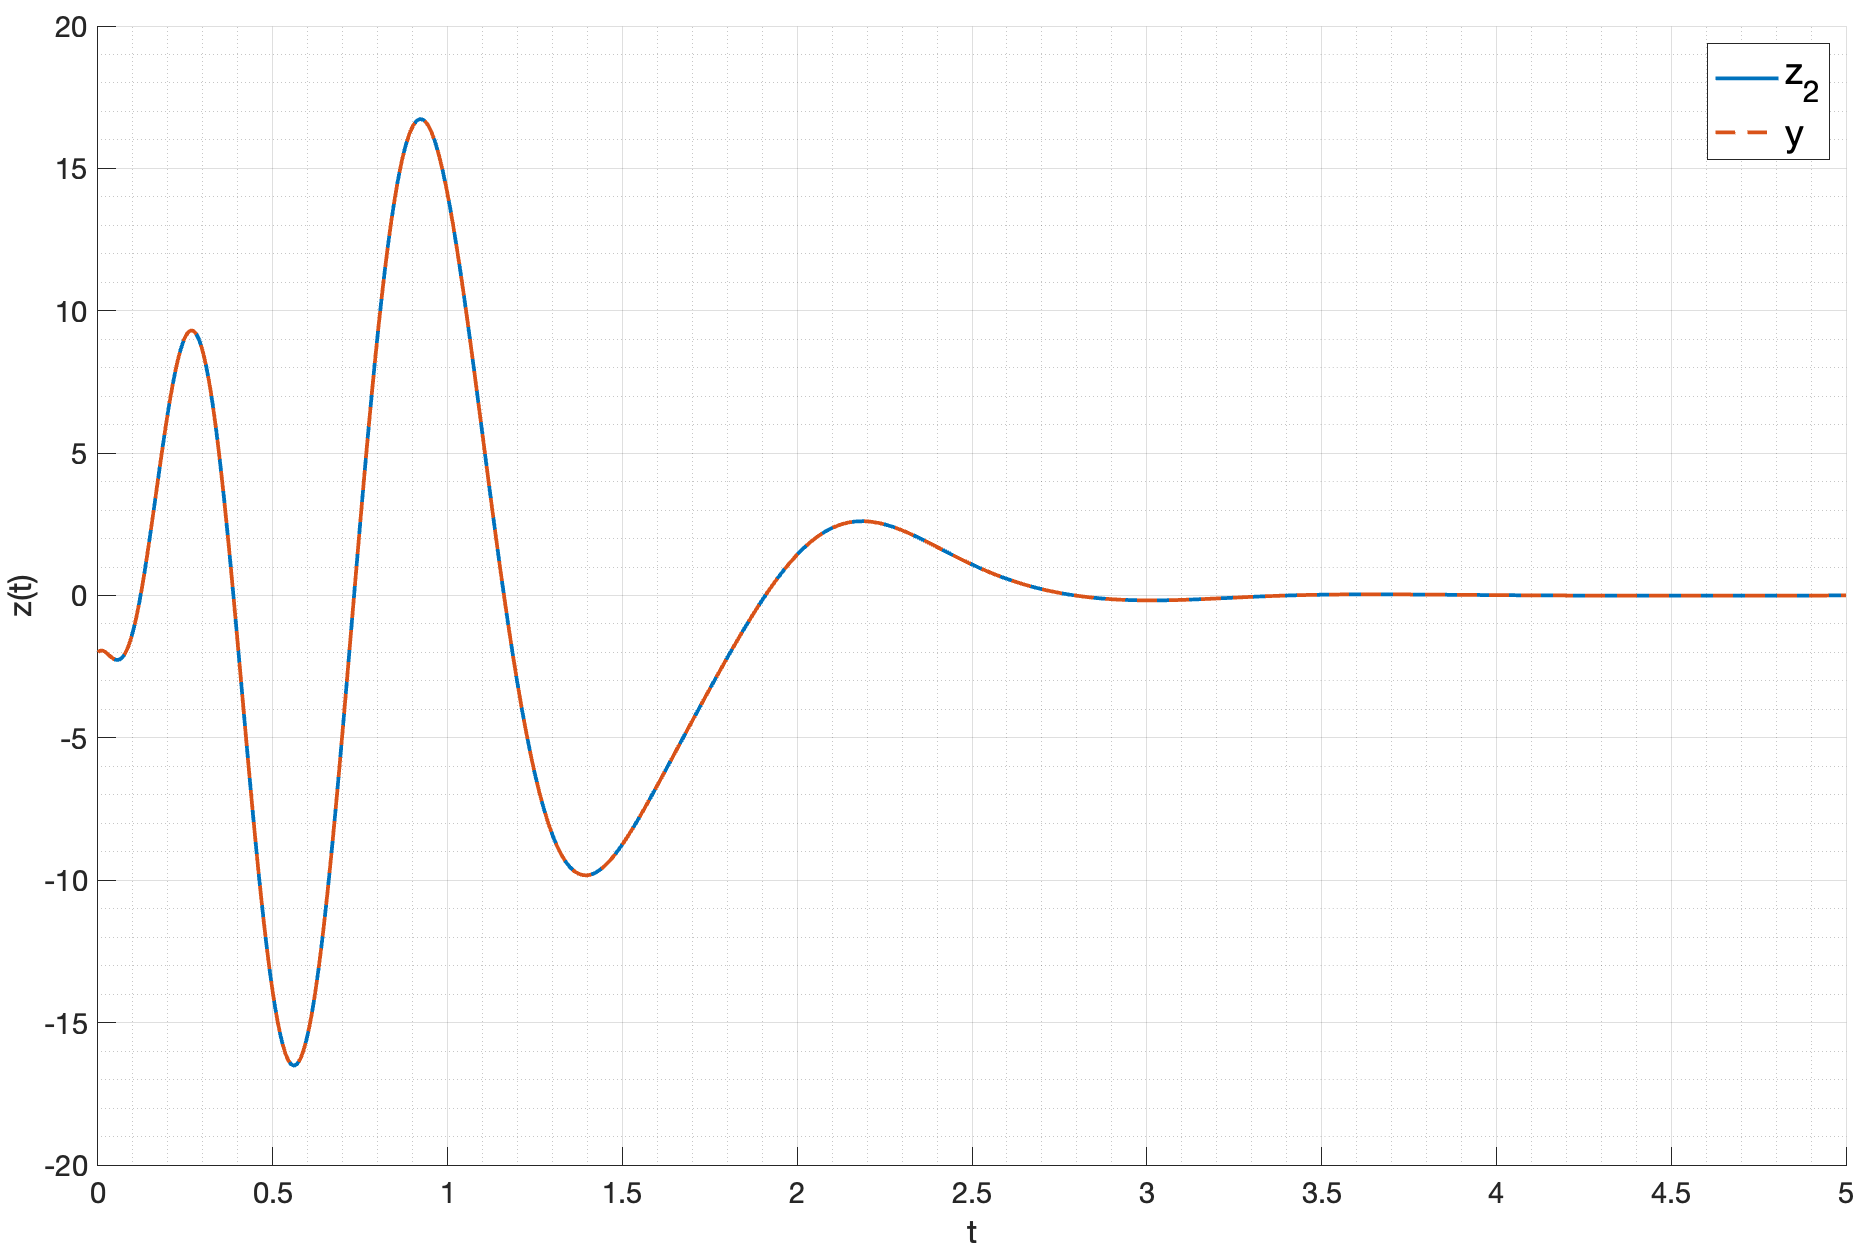
\includegraphics[width=\textwidth]{media/plots/task3_z2_cmp.png}
    \caption{Сравнение фактического и виртуального выхода системы}
    \label{fig:task3_z2_cmp}
\end{figure}
В этом же случае видно, что фактический и виртуальный выходы системы совпадают, что подтверждает то, 
что система имеет полную модель генератора внешнего возмущения и может полностью
компенсировать его.

\FloatBarrier

\subsection{Выводы}
В данном пункте была рассмотрена система с внешним возмущением, которая замкнута 
регулятором на основе оценки состояния системы и внешнего возмущения расширенного наблюдателя.
Данный регулятор более реалистичен, так как в реальности иметь данные о внешнем возмущении практически 
всегда невозможно, что делает его более универсальным. По графикам видно, что система все 
так же стабилизируется, а регулятор справляется с задачей слежения за входным воздействием. 